\chapter{Introduction}\label{introduction}

\settowidth{\epigraphwidth}{Wonderful life : the Burgess Shale and the nature of history}
\epigraph{%
Without hesitation or ambiguity, and fully mindful of such paleontological wonders as large dinosaurs andAfrican ape-men, I state that the invertebrates of the Burgess Shale, found high in the Canadian Rockies in YohoNational Park, on the eastern border of British Columbia, are the world's most important animal fossils. Modern multicellular animals make their first uncontested appearance in the fossil record some 570 million years ago--and with a bang, not a protracted crescendo.}%
{\textit{\\Wonderful life : the Burgess Shale and the nature of history}\\\textsc{Stephen Jay Gould}}

The goal for this work is to determine the conditions under which robust, interesting, adaptive evolution can be started and undergo self-improvement in the non-living world. 

Ongoing evolution means something more than continual change of population frequencies; instead we refer to the goal of a process that continues to produce interesting, novel, and creative results, as does natural biological evolution; in other words, we mean the \textit{evolution of evolution.} Finally, we constrain our domain to software rather than wetware or hardware; simulations and models, rather than elements embedded in the physical world.

Natural evolution is the foundation for several related bodies of literature, in Computational Intelligence and Artificial Life, as well of course of the study of evolution in natural systems. As many have observed, there are major differences between the original inspiration and the spin-offs. Biological evolutionary systems are complex, contingent, emergent, endogenous and general. By contrast, artificial evolutionary systems such as Evolutionary Algorithms are exogenous, problem-specific and designed.

A convenient shorthand capturing these differences labels the biological inspiration as bottoms-up or emergent and the derived fields as top-down or designed. If the top-down approach has failed, then perhaps there might be mileage in returning to biology, our sole example of a general self-improving, self-organizing system.

But as biology is contingent, what is the most useful starting point for a recapitulation? Assume first of all that we are in the domain of software, rather than hardware or wetware, for practical reasons. And also assume that biological evolution does not depend upon embodiment - that the outcome can be adequately modelled at a conceptual level without being grounded in either the physical world, or in contingent biology such as enzymes, proteins and genes.

Then our belief is that the evolution of evolution itself can and will emerge under certain conditions, and that an emergent approach will be more successful than the predominant design-driven top-down approach today.


%Simple ongoing evolution is not the same as creative or interesting evolution; the current state-of-the-art is both insufficient and unsatisfying. \parencite{Bourrat2015} makes a related distinction between distributive and transformative forms of evolution, where distributive evolution sees simply a change in population distribution without the generation of novelties or new elements characteristic of transformative evolution. The fundamental open problem is how to achieve transformative evolution in artificial systems.

\emph{A copy mechanism with adjustable fidelity can auto-adjust for example to changing environmental conditions.}

\begin{itemize}
	\item
	      Not same as ENS--that explains natural processes; our goal is to achieve something that is as interesting in a different domain
	\item 
	      Not same as EAs--EAs have exogenous fitness, not open-ended (search through a fixed space, cannot surprise (e.g., \parencite{Nellis2014})
	\item  
	      Not same as approach where take ideas from biology and evaluate for different purpose (e.g., in EAs, island populations, GRNs (e.g., L-systems), Lamarkian learning, co-evolution, evolutionary transitions (cooperation and mediation in \parencite{Defaweux:2005fk}\ldots{}). All seem to follow model of currently we use these tools, biology has something we don't have, let's try it\ldots{}
	\item
	      Not the same as most type of Alife, where evolution is not the subject of the research but rather a tool or mechanism towards some other goal (canonically, creating artificial life.)
\end{itemize}

\section{Motivation}

\epigraph{%
In the world of human thought generally, and in physical sciences in particular, the most important and most fruitful concepts are those to which it is impossible to attach a well-defined meaning.}%
{\textsc{\\H.A. Kramers}}

Natural evolution is the best example we have today of a transformative, adaptive improvement process. Many fields would benefit from a robust general optimisation heuristic for use when exact methods are not possible, and the example of natural evolution is our current gold-standard. 

As stated by many (\eg \parencite{Pascal2013}) a definition of life is elusive, and probably not useful. There is no definite boundary between the living and the non-living; as \parencite{Pascal2013} goes on to explain, the most likely scenario for the origin of life is that there was a series of intermediates, of increasing degrees of ``aliveness''. The corollary is that it is hard therefore to imagine a clear cut transition between non-living and living. Think of a present day virus--is it alive, or not? Reproduction is generally thought of as a requirement for life, yet viruses cannot reproduce without co-opting the necessary machinery from an independent host. 

\parencite{Fernando:2007pf} presents a partial compendium of definitions which illustrates the range of opinion:

\quote{
...at least one of the following outcomes: ‘open-ended evolution’ (Bedau et al., 2000); the origin of basic autonomy, i.e. a dissipative system capable of the recursive generation of functional constraints (Ruiz-Mirazo et al., 2004); a process ultimately capable of the production of nucleic acids or other modular replicators with unlimited heredity potential (Maynard-Smith and Szathmary, 1995; Szathmary, 2000); identification of ``the course of evolution by which the determinate order of biological metabolism developed out of the chaos of intercrossing reactions'' (Oparin, 1964); the coupled cycling of bioelements (Morowitz, 1968, 1971); the maximization of entropy production by a biosphere (Kleidon, 2004); the minimal unit of life (Ganti, 2003a, b); or an autopoetic unit (Maturana and Verela, 1992)?}{\parencite{Fernando:2007pf}}

One interesting distinction between living and non-living comes from \parencite{Rasmussen2004}--non-living systems explore a state-space driven by thermodynamics, and so in a sense through a random ergodic search. Living systems however almost universally employ evolution. Another information-theoretic view, from \parencite{Adami2015}, is that living systems can preserve information on a much longer timescale than non-living things. Given the relationship between information and entropy, the statement about metabolism in \cite{Schrodinger1944}--how ``living matter evades the decay to equilibrium''--seems very similar.

\begin{figure}
\begin{framed}
%\epigraph{%
%``What we do not know today we shall know tomorrow. A whole army of biologists is studying the structure and organization of
%living matter, while a no less number of physicists and chemists are daily revealing to us new properties of dead things. Like two parties
%of workers boring from the two opposite ends of a tunnel, they are working towards the same goal. The work has already gone a long way
%and very, very soon the last barriers between the living and the dead will crumble under the attack of patient work and powerful scientific
%thought.''}%
%{\textit{\\The Origin of Life}\\\textsc{Alexander Oparin}}

%Darwin ``warm little pond'' Life and letters vol3 1887
%(``\emph{\textbf{But if (and Oh! What a big if!) we could conceive in
%	some warm little pond, with all sorts of ammonia and phosphoric salts,
%	light, heat, electricity etc, present, that a protein compound was
%	chemically formed ready to undergo still more complex
%	changes\ldots{}'')}} \parencite{Vasas2012}

Tthe evolution of life was almost certainly contingent, and there is an absence of evidence from early stages \parencite{Pross2013}. There were many possible pathways, and unless some record remains somewhere (either geological or phylogenetic), the actual path is essentially lost to history. So without evidence for historic aspect, it is not possible to test hypotheses by falsification, and hence they can only be speculative.

However, a consensus is forming that early life began with chemoautotrophs fueled by energy from inorganic redox couples and biomass from CO\textsubscript{2}, and that innovations in carbon-fixation created the main branches in the tree-of-life \parencite{Braakman2012}. Initiation of selection marked by \gls{ida}, probably from RNA world, followed substantially later by Last Universal Common Ancestor (LUCA) \parencite{Yarus2011}, which, it is important to note for clarity, was almost certainly not a single cell or even species, but rather a construct of evolutionary genetics because of the likely predominance of Lateral Gene Transfer (LGT) in archaic biology (http://sandwalk.blogspot.ca/2007/03/web-of-life.html).

Self-replicating RNA enzymes shown in \parencite{Lincoln2009}, forming basis of selective system (link to natural selection) (also see \parencite{Cheng2010}, \parencite{Powner2009} for formation of RNA in prebiotic conditions). Some elements of \gls{ida} thought still with us in lineages of informational (for protein synthesis and RNA transcription) and operational genes (for some standard cellular processes) \parencite{Ragan2009}, for example the ribosome and ribonuclease P (RNase P) \parencite{Wilson2009}. Next major transition to Protein world (although predominance of RNA transcripts leads to suggestions that should be called RNA-Protein world \parencite{Altman2013}). Note however that Lateral or Horizontal Gene Transfer thought to have been so common in early life that there was no single common ancestor, but genes from multiple lineages combined into all lineages today.\parencite{Ragan2009}

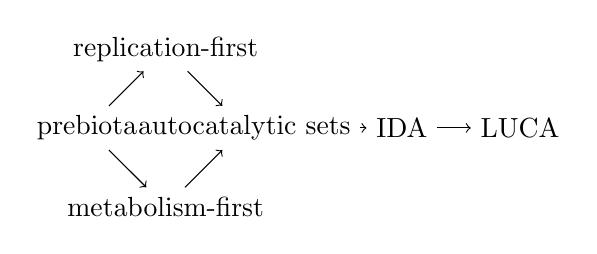
\begin{tikzpicture}
\node (prebiota) at (0,0) {prebiota};
\node (metabolism-first) at (1,-1) {metabolism-first} edge [<-] (prebiota);
\node (replication-first) at (1,1) {replication-first} edge [<-] (prebiota);
\node (acs) at (2,0) {autocatalytic sets} edge [<-] (replication-first) edge [<-] (metabolism-first);
\node (ida) at (4,0) {IDA} edge [<-] (acs);
\node at (5.5,0) {LUCA} edge [<-] (ida);
\end{tikzpicture}

Two alternative models exist for the step from abiotic to \gls{ida}: genetic or replicators or RNA-first, and metabolism or protein-first. Both metabolism and replication were almost certainly required for \gls{ida} however. A self-sustaining autocatalytic network (in terms of a RAF set specifically a ``set of molecules and reactions which is collectively autocatalytic in the sense that all molecules help in producing each other (through mutual catalysis, and supported by a food set).'') generally considered essential \parencite{Pross2013}, but not sufficient \parencite{Hordijk2011}. Both competing models--replication first and metabolism first--build on that. Autocatalysis expressed by self-replication of oligomeric compounds in replication first; by cycles and network in metabolism first. In the broadest sense, life can be seen as an autocatalytic process where an entity catalyses the production of one or more descendant entities.
From another perspective, Metabolism-first privileges function, while replicator-first privileges descent.

The main issues with replicator-first model are the sizeable step required from abiotic compounds to template-based replication (although ribonucleotides conceivably could form in pre-life conditions see \parencite{Powner2009}). Templates encode information in biology, so require a encode/decode mechanism as well as an information code to represent the product. This is a step more complex than simpler duplication. By contrast, the main issue with metabolism-first model concerns the shift from composome inheritance to template-based, and the ability of composomes to fulfill heredity requirement for natural selection.

The origin of life can be seen as the transition from chemistry to biology, and is analogous to our goal of transitioning from simple uninteresting systems, to systems which evolve. However, the usefulness of the similarity is limited: the primary postulates of OOL are not our postulates. Some abiogenesis results fundamentally assume real-world chemistry and
conditions, a constraint that doesn't apply to Alife or artificial OEE, and so is more restrictive than required. Other abiogenesis work such as on properties of autocatalytic sets, or the suitability of the genetic and catalytic properties of RNA for Alife \parencite{Cheng2010}, is broader in applicability.
\end{framed}
\captionsetup{name=Box}
\caption{The origins of life}
\label{box:ool}
\end{figure}

\subsubsection{Living organisms are supremely well suited to their environments, and can adapt to environmental changes}

Adaptation of organisms to their environments occurs in the main on two different time-scales.

Evolution by \gls{naturalselection} acts over a period of generations on populations of individual organisms. Changes are therefore relatively gradual, and many generations can pass before a change such as a beneficial mutation becomes ubiquitous in a population (\eg 300-500 generations for targeted modifications in lactose processing in \emph{E. coli} \parencite{Dekel:2005fk}. In contrast, gene regulatory effects act during the life cycle of a single individual, either during development to affect morphology, or during the adult lifespan in reaction to seasonal or other environmental cues. These regulation-driven changes are not in themselves heritable, but they can be assimilated back into the population by influencing the organisms fitness under natural selection (\eg,\parencite{Baldwin:1896ly,Dennett:2003ve,Paenke:2009xe,Paenke:2007ve}).

Similar effects can be seen by another adaptive mechanism that operates on individuals during their lifespan: learning, where behavioural adaptions can also lead to genetic change (\eg \parencite{Hinton:1987vy}.)

\subsubsection{Natural selection, acting on populations, is the primary driver for long-term adaptation}

The year 2009 saw the celebration of the 150\textsuperscript{th} anniversary of the publication of \emph{On the Origin of Species}, the explanation of evolution by natural selection, with extensive coverage in scientific and popular media. The terms are therefore fairly well known to many people, but what exactly does \emph{natural selection} mean? To quote from \parencite{Futuyama:1979tg}, \gls{naturalselection} is the ``differential survival and reproduction of genotypes''.

Let's examine each of the components in this idea in turn:

Differential survival. Living organisms are constantly engaged in an intimate relationship with their environments. Indeed, according to the theory of \emph{autopoiesis} \parencite{Varela:1974qd}, organisms are defined by this engagement: to be alive means maintaining oneself against the surrounding environment. In general the more effectively the organism is able to do this, the more likely it is to survive. However, in practice survival for an individual may be affected by random events. Scholarship winning students can be killed by drunk drivers. Sardines in shoals flash and turn, yet sharks still manage to grab one or two from the shoal effectively at random. Averaged over a population however these chance events balance out; a succession of random trials leads to a skewed distribution of fitness away from the less able.

Reproduction. In this sense, reproduction simply means inheritance. Only those characteristics that can be passed on from one generation to the next are relevant. One implication of this is that the only traits of an organism that matter to natural selection are those that are apparent while the organism can reproduce. Altruism and kin-selection, where an individual acts to increase the fitness of a related individual, are interesting for the light they shed on this implication.

Genotypes. An organism's \gls{genotype} is the heritable information that defines an individual, of which the great majority is encoded in DNA (some \emph{epigenetic} information is inherited through DNA-methylation, maternal protein concentrations and other mechanisms. However, generally DNA remains the primary source.)

How then does natural selection unfold in practice? Although an organism is defined by its genotype, its survival is based not on the raw genotype, but on the expression of the genotype--called the \gls{phenotype}--that participates in the interaction with the environment. There is not necessarily a direct one-to-one mapping between genotype and phenotype; for example, environmental triggers
during development can switch the phenotype in different directions (a phenomenon called \gls{polyphenism}.)

This indirect mapping enables a number of important mechanisms significant to the operation of natural selection: first, changes in the genotype (caused by mutations for example) may build up independent of phenotype changes--the idea of \emph{neutral mutations} \parencite{Ohta:1996vn,Ohta:2002ys,Ohta:1973kx}. Examples from studies of RNA secondary structures (the physical folding of RNA molecules) show that many closely-related RNA sequences can produce the same RNA folding \parencite{Fontana:1993zn}. Adjacent changes often have little effect on structure.

Second, by extension, \parencite{Gavrilets:1997qt} and \parencite{Gravner:2007yd} have shown that in cases involving many gene loci under well-defined conditions there is a path between viable phenotypes that requires only neutral mutations.

Third, behaviours such as learning, rather than purely genetic mechanisms, can influence the form of this \gls{gpmap} in combination with natural selection, as illustrated by the Baldwin effect \parencite{Baldwin:1896ly} and other examples of genetic assimilation \cite{Hinton:1987vy,Siegal:2002qn,Waddington:1942jb}.

Finally, a \gls{grn} provides another mechanism to modify the \gls{gpmap} and hence to guide natural selection.

\subsubsection{Novelties often arise from new regulatory connections rather than changes to genes}

The phenotype in living organisms is many orders of magnitude more complex than the genotype, and the methods used during development to build this complexity are many and various.

Cells call upon a complex of regulatory processes to regulate the expression of genes, and hence to control development and morphology (as well as to implement the cell's basic machinery.) The majority of these processes (at current understanding) use proteins to affect the initiation of transcription (the production of RNA from a segment of DNA, the first stage of gene expression); most commonly the presence of a specific protein promotes or inhibits the transcription of a related gene, and without transcription the gene is silenced.

One step further along the protein production chain, editing and splicing of the RNA products of transcription in eukaryotes prior to translation (the production of a protein from mRNA) is also under regulatory control. Many alternative proteins from one transcript can be produced, triggered by environmental or other influencing factors; each alternative protein will have a different effect on cell function. As a result, in biological organisms, the phenotype is not uniquely determined by the genotype, and a genotype contains the potential for multiple different phenotypes under the influence of the environment (a phenomenon known as plasticity).

Patterns of gene expression can also have an effect outside the originating cell, a phenomenon crucial for development. Signalling proteins produced by a cell act as regulators on the machinery of surrounding cells, and epigenetic mechanisms allow signal effects to be long-lived so that a pattern of expressions may be inherited by daughter cells without the continued presence of the original signals. These mechanisms determine the fate of new cells during development: a cell originating in an area bathed in a particular combination of signalling molecules will develop in a specific manner (such as into a skin cell); another cell in another area will receive different signals, and therefore develop in a different way.

The development of an organism from a zygote is thus controlled by a pattern of gene expression under the combined influence of a regulatory mechanism and the environment.

As the regulatory mechanism is constructed from proteins and RNAs encoded in the genotype, and as the genotype is generally under the influence of natural selection, evolution also acts upon gene regulation, and hence upon development. The study of the evolution of the developmental mechanism itself is known as Evolutionary Development, or, more colloquially, EvoDevo.

\parencite{Prudhomme:2007ax} believe that evolutionary novelties more commonly arise from changes or additions of regulatory \emph{connections} than from the development of \emph{new} genes or regulatory elements; that is, from changes to the network topology rather than from additions to the network elements. The underlying implication is that novelties are therefore new compositions of
pre-existing elements, rather than being constructed `\emph{de novo}', and that production of novelties may be relatively rapid. Connection changes may happen quickly; by comparison, new genes may take many generations.

\begin{flushright}
	\emph{According to the strictly structural concept, the genotype is considered as a mosaic of independent molecular blue-prints for the building of individual cellular constituents. In the execution of these plans, however, co-ordination is evidently of absolute survival value. The discovery of regulator and operator genes, and of repressive regulation of the activity of structural genes, reveals that the genotype contains not only a series of blue-prints, but a co-ordinated program of protein synthesis and the means of controlling its execution.}
	\par\cite[p354]{Jacob:1961ys}
\end{flushright}

A network formed by the regulatory interactions between genes and the transcriptional products of those genes (\glspl{tf}) is known as a Gene Regulatory Network, or \gls{grn}.

\subsubsection{Modularity is an emergent property of GRNs}
Even a superficial look at a set of randomly sampled insects reveals a striking level of similarity between supposedly distantly related species. Mouthparts, segmented bodies, wings and halteres springing from body segments, antennae on head segments; common patterns abound. The explanation lies in the action of a group of homeotic (or body-patterning) genes, which act in concert to impose a structure on the developing body plan. These regulatory genes, amongst the first patterning genes to be identified and characterised, in fact appear in very similar forms across all animals and hence appear to share a common evolutionary origin, and to be highly conserved \parencite{Shubin:2009vw}. 

As an example of their action, the gene \emph{Ubx}, or \emph{Ultrabithorax}, is involved in development of the \gls{metathorax}, one of the body segments, in \glspl{arthropod} \parencite[pg. 696-697]{Watson:2008fm}. Changes in \emph{Ubx} expression in combination with expression of a second homeotic gene, \emph{Scr}, are responsible for some of the differences in body plan between two arthropod groups - brachiopods, and isopods. In brachiopods, the expression of \emph{Ubx} suppresses \emph{Scr} in the leading thorax segment leading to development there of swimming legs. In isopods however, \emph{Ubx} expression has been lost in that segment, and instead a feeding appendage develops \parencite{Watson:2008fm}.

The morphological patterns that result from changes in expression of the \emph{hox} homeotic genes are textbook examples of modularity caused by regulatory networks. These networks in general appear to take a characteristic form, sometimes called a `medusa' network \parencite{Kauffman:2004zi,Aldana:2007da} where a regulatory head controls the expression of many functional genes. For example, in \gls{drosophila}, the medusa has a head of around 80 genes \parencite{Aldana:2007da}. \Textcite{Davidson:2006wi}, using the well-characterised sea urchin genotype, identifies GRN `kernels' of interconnected and hence very robust regulatory genes that control essential functions such as heart development and the endoderm specification in sea urchins. 

\section{Background and context}\label{background-and-context}

There has long been interest in understanding how biological evolution generates robust, novel, creative outcomes, unlike those seen in current artificial evolutionary systems. This has led to a drive towards understanding the fundamentals of biological evolution rather than in the historical inspiration of specific biological elements and structures, many of which are contingent and perhaps even arbitrary; certainly complex.

Related work falls into three main areas:

\begin{itemize}
\item Work specific to the overall problem: the conditions for the evolution-of-evolution in software systems.
\item Work related to the subproblem of a viable model for the evolution-of-evolution in software.
\item Work related to implementations of open-ended evolutionary systems in software.
\end{itemize}
	
This \namecref{background-and-context} expands upon previous work that is directly relevant to our overall problem, with the other two areas being reviewed in the Previous Work sections of the subsequent Parts of the thesis. 

The relevant open problems are summarized in the conclusion to this section.

\subsection{Evolutionary principles from Biology}

``We take it as given that biology instantiates ENS'', but that doesn't mean that the algorithm of biology is in fact \gls{ens} \parencite{Watson2012}. Adaptation in biology appears to precede Natural Selection, so adaptation is possible without \gls{ens} \cite{Watson2010}. \cite{Saunders1994}, discussing Lovelock's DaisyWorld model, explains how regulation can emerge in DaisyWorld without selection--the planet's temperature is adjusted to meet the conditions for maximum growth of the daisies without the daisies adapting to the planet. In fact, \cite{Saunders1994}, referencing Mayr, comments that Darwin could not prove that \gls{ens} was the only mechanism for adaptation in biology, just the most likely one. Subsequently, the developing understanding of the biology in areas such as \gls{hgt} and neutral theory \cite{Kimura:1968uq} has enhanced the purely Darwinian view of \gls{ens} in natural populations into what is now generally referred to as the modern evolutionary synthesis.

Although the advantages of a distinction between genotype and phenotype are discussed by many, including \parencite[section 7.2.3]{Taylor1999} and indirectly \cite{VonNeumann1966}, there is no inherent dependency on this in \gls{ens}. Early evolution may have involved holistic or composomal evolution before the advent of digital evolution with a separate genome.

\quote{Evolution is a process that results in heritable changes in a population spread over many generations.}{
	``Sandwalk: strolling with a skeptical biochemist'',
	\url{http://sandwalk.blogspot.co.nz/2012/10/what-is-evolution.html}}

\quote{
	Biological evolution consists of change in the hereditary characteristics of groups of organisms over the course of generations. Groups of organisms, termed populations and species, are formed by the division of ancestral populations or species, and the descendant groups then change independently. Hence, from a long-term perspective, evolution is the descent, with modification, of different lineages from common ancestors.}{``Evolution, Science, and Society: Evolutionary Biology and the National Research Agenda'', Working Draft, 28 September 1998, \url{http://www.zoology.ubc.ca/~otto/evolution/Evolwhite.pdf}}

\subsubsection{Evolution by Natural Selection (ENS))}\label{ens-evolution-by-natural-selection}

\cite{Godfrey-Smith2007} examined a number of summaries of \gls{ens} in the literature. The purposes of the summaries varied, but have interest for us ``as attempts to capture some core principles of evolutionary theory in a highly concise way.''. Incidentally, as an illustration of the difficulty of definitions, although the usual aim is to ``give conditions that are sufficient ceteris paribus for a certain kind of change occurring.'', \cite{Godfrey-Smith2007} notes that the scope of most summaries is somewhat ambiguous. They can be read as either being discriminatory--``this process is ENS''-- or providing conditions that will result in \gls{ens} when it is assumed that the meaning of \gls{ens} is clear. In other words, these are alternative \emph{constitutive} or \emph{causal} readings; in the example of \cite{Godfrey-Smith2007}, ``becoming pregnant\ldots{}{[}versus{]} being pregnant''.

Of these summaries, three are predominant:

\begin{enumerate}
\item
``Owing to this struggle for life, any variation, however slight and from whatever cause proceeding, if it be in any degree profitable to an individual of any species, in its infinitely complex relations to other organic beings and to external nature, will tend to the preservation of that individual, and will generally be inherited by its offspring. The offspring, also, will thus have a better chance of surviving, for, of the many individuals of any species which are periodically born, but a small number can survive. I have called this principle, by which each slight variation, if useful, is preserved, by the term of Natural Selection, in order to mark its relation to man's power of selection.'' \cite{Darwin1859}

\item
``if there is a population of entities with multiplication, variation and heredity, and if some of the variations alter the probability of multiplying, then the population will evolve. Further, it will evolve so that the entities come to have adaptations....'' (Maynard-Smith, in \cite{Griesemer2001})

\item
``1. Different individuals in a population have different morphologies, physiologies, and behaviors (phenotypic variation). 2. Different phenotypes have different rates of survival and reproduction in different environments (differential fitness). 3. There is a correlation between parents and offspring in the contribution of each to future generations (fitness is heritable).'' \cite{Lewontin:1970mc}

\end{enumerate}

From the study of the summaries, \cite{Godfrey-Smith2007} concludes that the core requirement for \gls{ens} is some ``combination of variation, heredity, and fitness differences'', although he identified a number of differences between the summaries. For example, the most commonly cited summary is \cite{Lewontin:1970mc}, but unusually that formulation states that ``fitness is heritable'' whereas typically phenotypic heredity (as appears in Lewontin's later 1980 summary) is stated as sufficient for a trait to evolve. 

These differences are also captured in \parencite{Griesemer2001}, in particular with reference to the variations between Darwin's concept of inheritance in \cite{Darwin1859} which includes both heritability (a capacity) and inheritance (a process carrying the capacity); Lewontin, which stresses the heritability while assuming inheritance, and Maynard Smith's multiplication which is actually about inheritance; his heredity is both. \parencite{Griesemer2001}

Quite apart from these differences in interpretation, the major theoretical difficulty in a literal application of \gls{ens} to artificial systems is captured succinctly by \parencite{Griesemer2005}: ``Darwin's theory of evolution by natural selection is restricted in scope. One sense in which it is restricted is that it refers to organisms.'' Organisms are not defined, but the context and scope is clearly biological.

Pigliucci2008 - ``Is evolvability evolvable?''

\subsubsection{Compositional evolution}

In life, have \gls{hgt} e.g., \parencite{Ochman2000}; \parencite{Watson2002} discusses compositional evolution and building blocks; \parencite{Pross2011} introduces Dynamic Kinetic Stability as a general principle underlying evolution, and proposes it as the driver for the origin of life.

\parencite{Arthur2009} investigates the evolution of technology, where evolution is used in the sense of \quote{all objects of some class are related by ties of common descent from the collection of earlier objects.}{\parencite{Arthur2009}} In general though, Arthur's compositional evolution does not attempt to understand life, but instead as a guide to achieving similar property in another domain, or in understanding similar processes in another domain \parencite{Arthur2009}.

Evolution in technology occurs by using earlier technologies as building blocks in the composition of new technologies, and these new technologies then become building blocks for use in later
technologies, and so on. Arthur calls this ``combinatorial evolution.'' But what is the starting point? How is this regression grounded? Arthur proposes that the capture and harnessing of natural
phenomena starts each lineage, and provides new raw components for inclusion in later technologies.

Evolution is related to innovation: in fact, Arthur claims that by understanding the mechanism by which technologies evolve we will understand how innovations arise. In other words, innovations arise
as the result of an evolutionary process, rather than de novo from the brain of a designer. Darwinian evolution, or natural selection, is not appropriate for technology. Arthur quotes from Samuel Butler's essay ``Darwin Among the Machines'' : ``{[}t{]}here is nothing which our infatuated race would desire more than to see a fertile union between two steam engines\ldots{}'' to illustrate the impossibility of slavish adoption of biological models.

The first obstacle to a more general scope is the existence of innovations such as the jet engine, laser, railroad locomotive, or QuickSort computer algorithm (to name Arthur's examples.) Innovations seem to appear without obvious parentage; they do not appear to be the result of gradual changes or adaptations to earlier technologies. Arthur's answer is to look inside the innovation and to recognise that each is made up of recognisable components or modules; the key lies in the nature of heredity in technology. Technologies are formed by combining modules of earlier technologies. These groupings start as loose assemblages to meet some new function, but over time become fixed into a standard unit (for example, the change in DNA amplification mechanisms from assemblages of laboratory equipment to standard off-the-shelf products.)

\parencite{Bourrat2015} comments that distributive evolution (where only the distribution of elements changes, as result of selection or drift) cannot result in novelties. Arthur's response is that novelty comes from incorporating new phenomena from the source, the natural world.

\subsection{Evolution in artificial systems}

The field of \glspl{ea} originated in the exploration of abstract biological evolution, but rapidly diverged into problem-solving and optimization \cite{De-Jong:1993gy,DeJong2006}. The fundamental differences between the biological original and the modern canonical \gls{ea} include:

\begin{itemize}
\item \Glspl{ea} search through a fixed space, and hence cannot surprise by 'kind', only by 'degree' (\eg \parencite{Nellis2014})
\item The evolutionary process in an \gls{ea} is not itself subject to evolution; it is designed, and a large body of literature exists to guide the implementor in the choice of algorithms to employ.
\item Fitness in an \gls{ea} is measured by an explicit \emph{objective function} whereas in biology fitness \emph{emerges dynamically} through continuous interaction with the environment. ``The difference is that we require a system with the potential for a large degree of intrinsic adaptation for open-ended evolution, rather than a system where the selection of individuals is determined by an externally-defined fitness function'' \parencite{Taylor2001}
\item \Glspl{ea} conduct a series of discrete trials of fitness, rather than a continuous evaluation.
\item Individuals in a \gls{ea} do not interact other than indirectly through a pre-designed selection mechanism.
\end{itemize}

The first two of these differences are significant; \glspl{ea} are not capable of open-ended, or evolutionary, evolution. However, recent research in biology continues to be applied to improve the performance of \glspl{ea} in their core function of optimization:
\begin{itemize}
	\item Redundancy and degeneracy--\eg \parencite{Whitacre:2010qy}
	\item Novelty--\eg novelty search \parencite{Lehman:2008cr}
	\item EvoEvo, or the evolution of evolution--\eg the remainder of this work.
\end{itemize}

For example, a summary of some relevant work in the application of \glspl{grn} to \glspl{ea} to improve the robustness and modularity of solutions can be found in \ref{applications-of-grn-in-eas}.

A form of re-unification between biological evolution and artificial evolution has been attempted in works such as \parencite{Paixao2015}, based on \quote{models in theoretical population genetics and in the theory of evolutionary computation}{\parencite{Paixao2015}}. For example: \quote{Some EDAs can be regarded abstractions of evolutionary processes: instead of generating new solutions through variation and then selecting from these, EDAs use a more direct approach to refine the underlying probability distribution. The perspective of updating a probability distribution is similar to the Wright--Fisher model.}{\parencite{Paixao2015}}



\section{Guide to this work}

\section{Previous publications}\label{previous-publications}

A version of Reactant and Product Strategies \cref{reactant-and-product-strategies} was published as \cite{Young2015},
and material from \cref{model-validation} in \cite{Young2013}.

ToyWorld is available under an GNU GPL v2 open source licence from GitHub \cite{toyworld}.

\section{Contributions}\label{contributions}

\begin{enumerate}
	\item
	Open-sourced Artificial Chemistry model
	\item
	Progress towards useful heredity in an artificial system
	\item
	Progress towards OEE in artificial system--evolution compatible with
	OEE without necessarily showing OEE (which is hard to measure and
	prove)
	\item
	Demonstration of formation of ACS in an artificial chemistry (previous
	work with ODEs e.g. \parencite{Hurndall2014} not re-usable in that form)
\end{enumerate}
\chapter{Previous work}\label{previous-work}

\epigraph{%
	It may appear that the properties one would have to assign to a population of self-reproducing elements in order to obtain Darwinian evolution are of a spectacular simplicity. The elements would only have to: (1) Be self-reproducing and (2) Undergo hereditary changes (mutations) in order to permit evolution by a process based on the survival of the fittest.}%
{\textit{\\Nils Barricelli}\\\textsc{Cited in \cite{Taylor2001}}}

Geb \cite{Channon:iw,Channon:2001ly} is claimed to be open-ended: artificial organisms controlled by neural networks created by a developmental process from a bit-string genotype. Individuals interact with the world through five predefined types of interaction generated by the neural network - reproduce (crossover and mutation of production rules), fight, turn anti-clockwise or clockwise, move forward. But the use of predefined interaction types, and the lack of a self-referential evolutionary model undermine this claim.

Everything in our artificial world must be built from a common set of raw materials; a loop connects the targets of selection with the environment. Other work, although superficially similar in that it models objects of similar scale, uses different models for the objects and the world (see \parencite{Sanchez-Dehesa:2008uq}) and so lack this loop.


``An important property of most strong AL systems is that they contain the ability for self-reference. For instance, Ray's Tierra organisms are able to read, copy, and modify their own code. In Fontana's algorithmic chemistry every object is a character string able to process other objects by using the lambda-calculus that maps the character string into an (active) function. The dualism inherent in those systems can be traced back to Godel who defined a mapping of mathematical statements into natural numbers `` that allowed self-reference, to Turing's universal machine, and to von Neumann's stored program computer .''\parencite{Dittrich1998}

``The term self-evolution should refer to an evolutionary process within a population system where the components responsible for the evolutionary behavior are (only) the individuals of the population
system itself. Every variation is carried out by the individuals. Selection pressure is generated implicitly through interaction among the individuals and not by external agents. The system must not contain a component that can be identified as a fitness function or global operators performing selection or variation (e.g., crossover).'' \cite{Dittrich1998}

Much of this work falls under the banner of \gls{alife}, both weak and strong as distinguished by \cite{Langton1989}: ``study the phenomena of life, not by simulating life as it is (weak AL) but by instantiating life as it could be (strong AL)''

First, a distinction: open-ended evolution refers to a goal or result, while evolution-of-evolution, or EvoEvo, describes a process or mechanism. The first is constitutive, the second causal. In artificial systems, the most influention formulation of the problem overall remains that of \cite{Bedau:2000mi}:

\quote{A key challenge is whether digital systems based on symbolic logic harbor the same potential for evolutionary innovation as physical systems. A preliminary challenge is to unlock the full potential of evolution in digital media. Many believe that digital life today falls far short in this regard, and this issue is starting to be approached quantitatively.}{\cite{Bedau:2000mi}}

\section{Recognition of open-ended evolution - consitutive definitions}

\parencite{Taylor2001} like others makes a distinction between OEE and ``kinds of evolutionary innovation''. He gives as an example of limited innovation the emergence of paratism in \cite{Ray1991} as direct result of system design and initial seeding conditions. In this reading, ``fundamentally new'' (labelled by Taylor as ``creative'') means new ways of sensing the environment and interacting with it \cite{Taylor2001}.

\quote{by open-ended evolutionary capacity we understand the potential of a system to reproduce its basic functional-constitutive dynamics, bringing about an un-limited variety of equivalent systems, of ways of expressing that dynamics, which are not subject to any predetermined upper bound of organizational complexity (even if they are, indeed, to the energetic-material restrictions imposed by a finite environment and by the universal physico-chemical laws)}{\cite{Ruiz-Mirazo2004}}

\begin{itemize}
	\item An open-ended evolutionary system must demonstrate unbounded diversity during its growth phase.
	\item An open-ended evolutionary system must embody selection.
	\item An open-ended evolutionary system must exhibit continuing (``positive'') new adaptive activity.
	\item An open-ended evolutionary system must have an endogenous implementation of niches.
\end{itemize} \cite{Maley1999} (considered ``rather abstract'' by Hutton \parencite[p.341]{Hutton2002}).

``openendedness depends fundamentally on the continual production of novelty.'' Standish, in \parencite{Soros2014}

``we would like the evolutionary system, like life, to continue to produce individuals of increasing complexity and diversity.'' -
although note, following McShea, that much of life is single-celled and hasn't become much more complex in billions of years \parencite{Maley1999}

\quote{by open-ended evolutionary capacity we understand the potential of a system to reproduce its basic functional-constitutive dynamics, bringing about an un-limited variety of equivalent systems, of ways of expressing that dynamics, which are not subject to any predetermined upper bound of organizational complexity (even if they are, indeed, to the energetic-material restrictions imposed by a finite environment and by the universal physico-chemical laws.}{\parencite{Ruiz-Mirazo2004}}

\section{Conditions for open-ended evolution - causal definitions}

Open-ended evolution can be seen as the outcome of evolution in an open-ended system (\eg Chemistry), where an open-ended system has effectively unrestricted representation: the number of possible types must be much larger than the number of individuals (ideally without any restriction). In the terminology of \cite{Szathmary:2006ty}, these are unlimited replicator (in contrast to limited replicators where the number of possible types is less than the number of individuals.)

Without this property all possible types can be generated in a finite time, and the system will either reach stasis or begin to repeat. Not all open-ended systems necessarily support evolution, but in those that do, our intuition suggests that open-ended evolution produces increasing complexity, increasing diversity, accumulation of novelty and continual adaptation \cite{Lehman2012}.

\Textcite{Taylor2001,Taylor:1999sc} discuss creativity in \gls{oee} in depth and argues that, for it to be possible, the replicators must \parencite{Hutton2004}:
\begin{enumerate}[label=\roman*] 
	\item Be fully embedded in their arena of competition 
	\item Have rich, unlimited interactions between each other and with their environment 
	\item Initially replicate implicitly, rather than using some encoding of the replication process, and 
	\item Be constructed entirely of `material' components, allowing the possibility of different encodings of information. (\quote{the very stuff from which they are constructed is a valuable resource of matter and energy}{\cite[s3.6]{Taylor2001}})
\end{enumerate}

\parencite{Taylor2001}:
Competition between individuals for resources - VanValen1973 Red Queen
hypothesis - primary source of intrinsic selection pressure.
Individuals and environment mutually affect each other

Resources must be ``(a) a vital commodity to individuals in the population; (b) of limited availability; and (c) that individuals can compete for (at either a global or local level). This resource can usually be interpreted as energy, space, matter, or a combination of these.''

``the potential for a large degree of intrinsic adaptation''

Ray made similar arguments in favour of interactions with other individuals (rather than isolated as in EA) 		

\parencite{Soros2014} presents four necessary conditions for OEE (it is left open if these are also sufficient conditions):
\begin{itemize}
	\item A rule should be enforced that individuals must meet some minimal criterion (MC) before they can reproduce, and that criterion must be nontrivial.
	\item The evolution of new individuals should create novel opportunities for satisfying the MC
	\item Decisions about how and where individuals interact with the world should be made by the individuals themselves.
	\item The potential size and complexity of the individuals' phenotypes should be (in principle) unbounded.
\end{itemize}
Along with these specific conditions, \parencite{Soros2014} assumes certain general conditions: a ``good'' genetic representation, a ``sufficiently large world for every individual to be evaluated'', and a seed or starting point.

Minimal conditions for OEE \parencite{Vasas2015}:
\begin{itemize}
	\item
	Very rich combinatorial generative mechanism e.g., organic chemistry.
	\item
	Unlimited heredity - number of possible heritable types should astronomically exceed individuals in population (Maynard-Smith:1995lw).
	\item
	Inexhaustible fitness landscape - implies rich, dynamical environment.
	\item
	Cannot state in advance possible preadaptations.
\end{itemize}

Bottom-up models for open-ended evolution leverage the richness of underlying environment - less information in entity definition, more in environment definition. Similar to biology, where physics and chemistry underpin living organisms, where definition of minimal cell many orders of magnitude simpler than the working out of the chemical and physical rules that it relies upon.

Top-down models assume a knowledge of the necessary elements.

``From the point of view of the evolvability of individuals, the more embedded they are, and the less restricted the interactions are, then the more potential there is for the very structure of the individual to be modified. Recall that this is one aspect of my definition of creative evolution. Sections of the individual which are not embedded in the arena of competition are `hard-wired' and
likely to remain unchanged unless specific mechanisms are included to allow them to change (and the very fact that specific mechanisms are required suggests that they would still only be able to change in certain restricted ways).'' \cite{Taylor2001}

Similar to the semantic closure of \cite{Pattee1995a}--``organisms should be constructed `with the parts and laws of an artificial physical world''' \cite{Taylor2001}

\parencite{Maley1999}

Focus on diversity (to make progress). Some suggestions previously that diversity is bounded (at minimum, by
number of molecules available for biosphere, also by energy and
minimal populations and probably other things), and plateaus
(punctuated equilibrium). Indicates two time constants - a fast expansion to use available resources, with a slower rhythm of innovations to create and enter new adaptive spaces.

Maley builds up the requirements by beginning with almost the simplest model possible (called Urmodel 1) where the only changes in the population from generation to generation are 1-bit flips in a 32-bit genotype. This results in a neutral fitness landscape (as no selection) and to prevent edge effects each run was stopped before all niches were filled. The, unsurprising, result was unbounded diversity, but no selection or heritable effect on fitness.

Posits that need selection : ``Requirement 2 An open-ended
evolutionary system must embody selection'' - because ``fails to meet
one of the basic criteria of natural selection: the heritable
variation has no effect on fertility'' {[}ignoring use of fertility as
a fitness-analogue{]}, and from Bedau ``Requirement 3 ...continuing
(`positive') new adaptive activity'' {[}ignore neutral theory, and
accepts Bedau - perhaps to allow use of Anew as measure?{]}

Urmodel2 - natural selection: mutation, ``dissimilarity'' for
competitive advantage (justified by biological example of niche
overlap theory (Levins, 1968)) - no increase in Anew

Urmodel3 - selective sweep (hypothesis): parasites (mutations) and
hosts (fixed genotypes). Fitness on degree of match between parasite
and host bit patterns.

\begin{itemize}
	\item
	
	Claim shows unbounded activity - ``the first known artificial
	evolutionary system demonstrating unbounded evolutionary activity''
	
	\item
	
	Restricted by 32-bit genomes, no death
	
	\item
	
	But probably not a unique or even significant result - ``The only
	trick is to defer the point when the model hits its true asymptotic
	behaviour for long enough that the growth dynamics of the model are
	themselves asymptotic in some sense''
	
\end{itemize}

Urmodel4 - ``the most important aspect of an organism's environment
are the other organisms with which it interacts'' - add coevolution to
Urmodel3 by letting hosts mutate

Two ``distasteful aspects of Urmodel3'' leading to belief that metrics
aren't right

\begin{itemize}
	\item niches are imposed from outside, not endogenous - this becomes Requirement 4
	\item no surprise - claim is because not complex - ``A puddle of inert,
	multicoloured and diverse algae would not be nearly so inspirational
	as the rain forest.'' Again, a biological metaphor.	
\end{itemize}

The EvoEvo project (\url{http://evoevo.liris.cnrs.fr/about-evoevo-project/}), an Information and Communication Technologies initiative funded by the European Commission, begins at a higher level biological starting point (genotype-phenotype mappings). The project presupposes microbial evolution, ``at the level of genomes, biological networks and populations.'', with a focus on four specific properties of a genotype-phenotype mapping - Variability, Robustness, Evolvability, Open-endedness. Later work is planned to remove the biological specificity to provide a framework for applying EvoEvo to ICT problems. Along with development of a model founded on the ``genotype-to-phenotype mapping and the fitness landscape'', the project states that make use of \emph{Aevol} \parencite{Knibbe:2006vn,Knibbe:2007kx} to model developmental processes in microorganisms.

\emph{Aevol} describes the genotype-phenotype map of an artificial organism modelled closely on a prokaryotic cell. The genotype is therefore made up of a \emph{double-stranded circular} bit-string with genes marked by promotor sequences and terminated by sequences that can form a ``stem-loop'' structure (where bases are arranged in sequence along a protein such that the binding between complementary bases causes a characteristic loop to form in the protein.) Expression levels of a gene are based on the degree of similarity between the gene's promotor sequence and a predefined ``consensus'' sequence (as calculated by the Hamming distance), as is the case in real-world prokaryotes where the basal transcription level depends on the quality of the promotor \parencite{Sanchez-Dehesa:2008uq}. Translation in \emph{aevol} takes place between marked regions of the gene, and proceeds three-bit codon by codon, with each codon translated according to an artificial genetic code into an amino-acid equivalent in a protein.

The \emph{aevol} model contains several innovations:

\begin{itemize}
	\item \emph{aevol} includes a proteome abstraction in the model in addition to the usual genotype and phenotype. Proteins in \emph{aevol} describe abstract ``processes'' instead of chemical interactions, where a process is described by a triangular probability distribution over $\mathbb{R}$ (in practice $[0,1]$ representing all processes) where triangles with positive height enhance the process and negative height processes act as inhibitors. The proteome then may be represented as either the superimposition of all protein distribution, or as the network of their ``functional interactions'' (the overlap between two protein distributions.) Note that the range of a process (protein) is equivalent to \gls{pleiotropy}; genes with a small range are functionally specialised. The phenotype of the organism is then the set of all positive processes (as calculated by Lukasiewicz fuzzy operators); that is, all activated but not inhibited processes.
	\item Mutations are not only the usual point-mutations (small deletions and insertions) but also \emph{genotype rearrangements}: deletions, translocations, inversions and duplications that act on a larger-scale.
	\item The environment for selection is also modelled by a similar distribution over $\mathbb{R}$. The closer the match between the organisms phenotype (as described above) and the environment distribution, the fitter the organism. This marks the full extent of environmental interactions in \emph{aevol} however. 
\end{itemize}

To study the relationship between regulatory processes and adaptation to changing environments \parencite{Sanchez-Dehesa:2008uq}, two major changes have been made to \emph{aevol} to give \emph{RAevol} or Regulatory \emph{Aevol} \parencite{Beslon:2010zr,Sanchez-Dehesa:2008uq}. The first is the implementation of a fine-grained time model; proteins concentrations now vary dynamically (instead of remaining static as in \emph{aevol}), and the organism's proteome and phenome change over time to reflect these protein changes. The other is the addition of a regulatory model. The calculation of the basal expression level of a gene in \emph{RAevol} is the same as that in \emph{aevol} - a function of the Hamming distance between consensus sequence and gene promotor sequence. However, in \emph{RAevol} this level is modified by the action of regulation, either up-regulating or down-regulating the basal expression. The degree of regulation is determined by the concentration of proteins that may bind to two regulatory sites (an enhancer site and an operator site for inhibition) each 20-bits long. The ability of a protein to bind to the binding site is calculated from a predetermined ``affinity'' matrix that mediates between the DNA bit-string representation of the binding site, and the amino-acid representation of the protein. A simple process change in \emph{RAevol} enables interaction with the environment:  during simulation, a signalling protein of set sequence that has no metabolic function but can act as a \gls{tf} is sent to the organism when the target environment changes.


Previous work is evaluated against three criteria: non-biological domain and purpose, emergence, and a self-referential or evolvable evolutionary mechanism.

\begin{table}
	\scriptsize
	\caption{Previous work}
	\label{tb:previous-work}
	\begin{tabular}{@{}lllll@{}}
		\hline\noalign{\smallskip}
		\Gls{achem}                                                        	& Type 	& Domain	& Emergent		& Self-referential Evolutionary mechanism\\ 
		\\ \noalign{\smallskip}
		\hline
		\noalign{\smallskip}
		\cite{Ducharme2012}                                             &Atoms/Molecules&&&\\
		StringMol \cite{Hickinbotham2012}                             	&Rewriting or String-based&&&\\
		Squirm3 \cite{Hutton2002,Hutton2007,Lucht2012}                	&Atoms/Molecules&&&\\
		RBN-World \cite{Faulconbridge2011}                            	&Boolean Networks and Graphs&&&\\
		\cite{Lenaerts2009}                                             &&&&\\
		ZChem \cite{Tominaga2009}                                     	&&&&\\
		Substrate-Catalyst-Link (SCL) \cite{Varela:1974qd,Suzuki2008} 	&&&&\\
		\cite{Fernando:2008xy,Fernando:2007pf}                             	&&&&\\
		\cite{Gardiner2007}                                                	&&&&\\
		NAC \cite{Suzuki2006}                                         	&&&&\\						
		GGL/ToyChem \cite{Benko2003,Benko2005}                        	&Atoms/Molecules&&&\\
		Lattice Artificial Chemistry \cite{Ono2000,Madina2003}        	&&&&\\
		Avida \cite{Ofria2004}                                  		&Assembler Automata&	Alife&	Yes&\\
		Tierra \cite{Ray1991}                                  			&Assembler Automata&	Alife&	Yes&\\
		Using Avida\cite{Lenski2003}									&Assembler Automata&	Both&	Yes&\\
		\cite{Taylor2001}												&&&&\\
		\cite{Antonakopoulos:2011th}									&Rewriting or String-based	&Alife	&Developmental 	&No\\
		\cite{Dittrich1998}												&Rewriting or String-based&&&\\
		\cite{Fenizio2000}\cite{Fenizio2001}							&Rewriting or String-based&&&\\
		\cite{Fontana1992}												&Rewriting or String-based&&&Yes\\
		\cite{Nellis2012}\cite{Nellis2014}								&Boolean Networks and Graphs&&&\\
		\cite{Segre1998}												&Compositional&&&\\
		\cite{Vasas2015, Vasas2012, Vasas2012a}							&Compositional&&&\\
		\cite{Kauffman1986}												&Compositional&&&\\
		Turing															&Rewriting 	&Alife	&Yes	&Yes\\
		Von Neumann														&&&&\\
		Waddington														&	Biology&&&\\
		\hline
	\end{tabular}
\end{table}

\section{Simulations of the evolution-of-evolution in artificial systems}

\parencite{Nellis2012}

``Our aim is to improve novelty-generation algorithms by making their biological models richer''

Novelty-generation as goal/theme for meta-evolution

No measure for novelty - not even sure is possible. But informal definition that says more novelty as result of more embodiment (this seems circular?) p87

Embodiment as mechanism. Provides overview in 3.2

AChems categorized as world/chemistry/constraints (p132), with constraints being energy model/binding model. RBN-World mentioned as a world where elements are RBN networks

States that binding model needs to be rich - empirical evidence presented (StringMol) only

Copying is a phenomenon, expressed through mechanisms at different levels of the AChem

Explored through embodied copying mechanism built in GraphMol, with antecedent in StringMol (Hickingbotham2011)

StringMol includes an embodied copying mechanism - start/at-end/char-copy/next. Some elements (at-end) use Smith-Waterman matching algorithm, which opens ability for evolution to modify the function of at-end (Nellis2012p143). But others, e.g., next, are not embodied. GraphMol makes next embodied

Design is graph based (obviously..). ``The world defined by GraphMol contains chemicals (represented as graphs) that bind to each other via multiple binding sites, and then run simple computer programs (encoded in the graphs) that modify the binding of these chemicals.''. Why? No explicit rationale presented. Presumably StringMol starting point meant programs, copying, then graphs? 
Operates (like StringMol) at level of proteins/enzymes e.g., replicases, DNA

Runtimes in weeks to months

\parencite{Nellis2014}

Summary of PhD thesis - computational novelty through embodiment

Comparing StringMol and GraphMol

Emergent systems easy to code but produce surprising results. Cannot predict results from rules (or in fact easily predict rules from desired results. One-way function, akin to encryption)

Standard GAs search through a fixed space - cannot surprise, limited range

Need something emergent

Mechanism of evolution must be itself evolvable; individuals and environment interact to give new ways of producing new individuals.
Dynamics required for novelty-generation.

Quick defined embodiment in terms of two dynamical systems mutually affecting each other - no need for a physical world. System modifies environment. Doesn't address if system is constructed from environment. Autopoiesis does say though that system built from environment. But autopoiesis talks about maintenance not evolution

Functions such as template copying must be embodied mechanisms in the world - so can be affected and evolved

Stringmol and Graphmol have embodied template copying, done in different ways. Different computational models result in different properties - ``Stringmol exhibits macro-mutation and two chemical copying; GraphMol exhibits two types of quasispecies, cooperative and parasitic. These two systems use the same domain (emergent evolution) and metamodel (machines copying strings), but different computational models.''

\section{Other potentially open-ended artificial chemistries}
\subsection{Assembler Automata}

Avida \parencite{Ofria2004}

``An approach to studying evolution...''

``According to Daniel Dennett, ``...evolution will occur whenever and wherever three conditions are met: replication, variation (mutation), and differential fitness (competition)''''

``(However, as Barton and Zuidema {[}3{]} note, general acceptance will ultimately hinge on whether artificial life researchers embrace or ignore the large body of population genetics literature.)''

Difference with GAs - natural organisms must replicate themselves to pass on genetic information - ``final arbiter of fitness'', and interaction with other organisms and with environment \parencite{Ofria2004}

Steen Rasmussen inspired by computer game core war - competing segments of simplified assembly code in core memory. With change to copy command to introduce mutations and hence evolutionary potential,
core world created. But system ``collapsed into a non-living state'' {[}non-living?{]} One possible reason - copying over existing organisms

Tierra next year (relationship not stated) organisms had to allocate memory first before using. Initial selective pressure only from rate of replication. Sequential execution of organism code

Avida summer of 1993 - better metering and measuring, and parallel code execution

``In principle, the only assumption made about these self-replicating automata in the core Avida software is that their initial state can be described by a string of symbols (their genome) and that they autonomously produce offspring organisms. However, in practice our work has focused on automata with a simple von Neumann architecture that operate on an assembly-like language inspired by
the Tierra system.''

Instruction, read, write, and flow control heads for relative rather than absolute addressing - bit like a Turing tape machine. Many instructions grouped into instruction sets. Default set has 26 instructions, and by definition every program is valid.
Phenotypes - ``The primary mode of environmental interaction is by inputting numbers from the environment, performing computations on those numbers, and outputting the results. The organisms receive a
benefit for performing specific computations associated with resources''
All very configurable, and complicated, but why? What rationale behind choices? More of a testbed for experiments, e.g., `` in one experiment we wanted to study a population that could not adapt, but that would nevertheless accumulate deleterious or neutral mutations through drift''
``The quest to halt adaptation is only one example of a special feature in Avida; many more have been explored, and are continuously being added to the source code. The most successful features are all fully described in the documentation that comes with the software.''

\parencite{Taylor2001}:
Derived from Thesis (Taylor:1999sc): creation of \gls{alife}, Extension of Tierra \cite{Ray1991} by cell regulation, parallel processes, energy modelling \cite[p.4]{Taylor:1999sc}, Cells are explicitly modelled as bitstrings which run as programs, and an adhoc theoretical model (essentially Tierra plus some previously identified improvements)
Phenotype fundamentally ``involves interaction with the environment (and that this is the essential distinction between the notions of phenotype and genotype - the latter being an informational concept)'' \parencite{Taylor2001}
Seed (proto-DNA) must itself be an indefinite heredity replicator {[}assumes that this is minimal starting point, rather than that this itself may evolve{]} \parencite{Taylor2001}
Assume that early stages see A+B implicitly encoded in the environment {[}essentially because simpler than explicit mechanism, but little justification{]} ``At the early stages of an evolutionary process, however, we would not expect there to be mechanisms for explicitly decoding the proto-DNA\ldots{}'' \parencite{Taylor2001}
		
\subsection{Rewriting or String-based}

\parencite{Antonakopoulos:2011th}

One developmental mapping for several structures or species e.g., CAs, and boolean networks - sparsely connected networks

Using L-systems - one for cells/nodes, and the other for connectivity rules

Developmental process ``capable of expressing developmental actions e.g., growth and differentiation'' and ``able to express a large variety of topologies within each architecture\ldots{}''

\cite{Dittrich1998}:
A simulation approach towards ``dynamic phenomena, especially on the emergence of prebiotic evolution'', based on an artificial chemistry, with advantages claimed over ODE approaches such as those in \cite{Bagley1992}

Introduction of  S,R,A classification scheme for artificial chemistry, where S=`` binary strings with a constant length of 32 bits'', R=s1+s2-\textgreater{}s3, and A=''simulates a well-stirred tank  reactor with mass-action kinetics, which assures that the probability of a collision is proportional to the product of the concentration of the colliding objects'' based on earlier work by Fontana and Kauffman.

A=``1. Select two objects s1,s2 from the soup randomly, without removing them. 2. If there exists a reaction s1 + s2 to s3 and the filter condition f (s1,s2,s3) holds, replace a randomly selected object of the soup by s3.'', s1 and s2 are not consumed, rather they act as catalysts. Chosen as this shown capable of hypercyclic organisation

AND reaction and an automata reaction to generate s3 from s1, s2. Automata is a deterministic FSA, running s1 (4-bit fixed instructions) on s2.

Measures (all macroscopic)

\begin{itemize}
	\item Diversity
	
	\item
	
	Distance Distribution Complexity (from Kim)
	
	\item
	
	Productivity
	
	\item
	
	Innovativity (innovation = new string)
	
\end{itemize}

\parencite{Fenizio2000}:

Original AlChemy reactions of form A+B-\textgreater{}C where C replaces an existing element (X)

This system generates A+B-\textgreater{}C1+C2...CN where C is a multiset of size N. Done by modifying the original K rule to detach x2 and eliminate both original elements (like reactants in chemistry)

Uses combinators rather than lambdas

To prevent from stopping (out of elements) added modification where randomly add/remove some elements

Combinator first combines (appends) elements, each element other than first bracketed. Then each 1-term combinator applied to string, where it makes specific changes e.g., K x1x2s0-\textgreater{}x1s0 (s0 is remaining substring, may be null). Apply until no further reductions possible (that is, in normal form). Two combinators are equivalent if can be reduced to same combinator (and previously noted that order is not important - same results regardless of order).

Free pool of atoms for conservation of ``mass''

\parencite{Fenizio2001}:

Experiment to show spontaneous formation of autopoietic cells, with a focus on ``identity as an entity separated from its environment'', that is, membrane formation. Graph used to model spatial structures: ``an artificial chemistry (AC) is embedded in a graph, with each molecule being a vertex of the graph and possible interactions being allowed only along the edges of the graph''. Molecules are composed of atoms taken from a 

``Molecules are built from a substrate of elements called atoms. There are seven types of atoms (I, K, W, R, B, C, S), each with a different function. The total number of atoms in the reactor is kept constant during a run. Free atoms (not bounded in molecules) are separately stored and form a global pool.''

As the rules for the combinations of two molecules are predetermined (the reaction mechanisms are described in \cite{Fenizio2000}), this model is not by our definition open-ended.

\subsection{Boolean Networks and Graphs}



\parencite{Faulconbridge2010, Faulconbridge2011}:

RBN-World \cite{Faulconbridge2011} chemistry where the entities are described as a form of Random Boolean Network, with the addition of a bonding mechanisms to allow for composition and decomposition of RBNs. A number of parameters affect the behaviour of the chemistry, and so a series of experiments sampled from the parameter-space, and then used a GA, to search for interesting variants as measured by non-catalysed ``loops'' (ideal measures of auto-catalytic sets and Hypercycles too rare for use as a measure) (\cite[§8]{Faulconbridge2011}). 

Entities are described as a form of Random Boolean Network, with the addition of a bonding mechanisms to allow for composition and decomposition of RBNs. A number of parameters affect the behaviour of the chemistry, and so a series of experiments sampled from the parameter-space, and then used a GA, to search for interesting variants as measured by non-catalysed loops (ideal measures of auto-catalytic sets and Hypercycles too rare for use as a measure) (chap 8)

Gillespie-like" - random reaction, random time - not correlated in any way with reaction energies or rates (Faulconbridge2011§8.4.3.1)

bRBNs used as atomic elements, properties determined by the network

Larger structures are formed by ``bonding'' two independent bRBNs at each bRBNs bonding node. ``All reactions are between two reactants; it is assumed that more complicated reactions can be expressed as a series of two-reactant reactions with intermediate structures.`` Record kept of composition so that decomposition can be easily done.

Many design choices - bonding mechanism etc. Examination of alternatives done by searching with EA

Each bRBN is a RBN, made up of a number of nodes, each with an initial state (true/false) assigned randomly and with a input/output matrix assigned randomly. Finally k(=2) inputs are established per node. Synchronous state update. All based on Kauffman1969 (interestingly, although noted as ``original'' so later work known) bonding method uses ''cycle length as the bonding property and equality as the bonding criterion....bonds only exist between bRBNs that have the same cycle length.'' in initial examples at least n=5 and b(k?)=2, and alternatives examined using EA. After initial bond formation recalculate cycle lengths, and check again for equality - might result in decomposition.

Describes two generic strategies for the selection of reactants, spatial and aspatial, where the primary difference is whether molecular position is a factor in reactant selection

Measures are Synthesis, Self-Synthesis, Decomposition, Substitution, and Catalysis (Faulconbridge2011§7), and non-catalysed `loops' (ideal measures of auto-catalytic sets and Hypercycles too rare for use as a measure) (Faulconbridge2011§8)

Random sampling + EA (Fitness function (§8.4.3.2) is based on non-catalysed loops (§4.3.9.4))		

"identifies three types of \textbackslash{}emph\{mixing method\} or reactor algorithm			

Contains an interesting discussion mapping these desirable properties onto the emergent properties that are then required of an \textbackslash{}gls\{achem\}

Some advantages claimed over Hutton (emergence and computational intractability p190)

``As the choice to use RBNs as the sub- symbolic representation in RBN-World was based on limited information. As a discrete dynamical system that is computationally tractable yet also spans a wide range of behaviours, RBNs met the appropriate criteria. It is not expected that RBNs are the best representation however; others may be more suitable for particular emergent properties.``

\subsection{Atoms/Molecules}

Ducharme et al \parencite{Ducharme2012}. The approach taken is to model the energy changes associated with reactions. The chemistry is spatial; atoms are arranged on a 2-dimensional grid and have velocity. When two atoms pass within a particular distance, they interact. The possible types of interactions are prespecified, with the type chosen being driven by the atomic composition and energies of the interacting atoms. Reactions are therefore between atoms rather than molecules; a molecule in this chemistry is a combination of atoms arranged in a particular structure, re-examined after each reaction to form a stable configuration based on expectations from real-world chemistry. Although computational costs are not reported, it seems plausible that the calculation of intersections on a 2-dimensional grid will be expensive for large molecular populations. Another cost comes from the re-arrangement of molecules into energy-efficient configurations. This spatial structuring enables the model to restrict atomic interactions to those atoms that are accessible on a molecule, but at the cost of additional modelling complexity. 

\cite{Fernando:2008xy,Fernando:2007pf}:
Driven by origin-of-life objectives (``the evolution of chemical networks that lead to autonomous systems'') so attempt to establish a phylogeny that includes first autonomous system
Simulation of laboratory experiment of lipid aggregates in a reactor. Strong theoretical justification. Hypothesis supported by inspection - single entities that are examples; Novelty is implicit in overall goals with sole quantitative measure (``fitness``) of integral of quantity and size - more and bigger is better
Molecules and food molecules share same representation and chemistry
Molecules, light-energy and thermodynamics
Hill-climbing algorithm replaces parent with first 10\% better-fitness child; explicit fitness calculation
Experiment reported in \textcite{Fernando:2008xy} generates phylogeny which is then examined and interpreted - danger of arguing from specific to general. Shows only possible, no more.

\parencite{Lucht2012}

Challenge to community - "to develop a system in which, starting with a soup of free atoms and a simple ``bootstrap'' chemistry, a cell-like creature similar to the one in H-41 evolves."

Based on Hutton2007 Squirm3 chemistry, using Hutton's floods 
Squirm3 - fixed molecule types, and pre-defined reactions for replication and gene-sequence transcription, and so although capable of interesting behaviour is not capable of unlimited extension

Added reaction types to address Squirm3's ``global-extinction problem and showing how quasi-universal enzymes can evolve''

\cite{Hutton2007,Hutton2002}:
Artificial system capable of life-like \gls{oee} (creativity).
Based on hypothesis (materiality, interactions, embedding) of \textcite{Taylor2001}, better expressed in \textcite[p.341]{Hutton2002}; membrane to allow individuals to benefit from innovations by protecting internal reactions from others.
\Gls{achem} from \textcite{Hutton2002} used to construct all elements in world - material and embedded.
Atoms in \gls{achem} of different types and states; reaction rules; otherwise no energy modelling; only physics modelling is the concept of location (either integer-coordinates or real number-coordinates) and impossibility of colocation. Floods are used to recycle raw materials.
Individuals (each bounded by a membrane) with the capability for division and mutation. Raw materials (atoms) are only required for division.
Interactions between individuals are limited to effects on shared environment (niche construction without direct interaction), so one element of hypothesis untested; restrictions on open-endedness: evolution of new enzymes unobserved as extremely unlikely, and genotype-phenotype mapping hard-coded (unevolvable)

Enzymes can act as catalysts so G affects P; but enzyme evolution too improbable for OEE

2D grid of squares (lattice), spring force for membrane

Enzymes can now affect all reactions except enzyme production; in practice too slow

Production rules hardcoded into AChem

Only with raw materials in environment, niche construction through adaptation to availability of raw materials

AChem hand-built with reactions instead of enzymes
Prespecified reactions - see Faulconbridge2011 p.49

Artificial system capable of life-like \textbackslash{}gls\{oee\} (creativity)

Based on hypothesis (materiality, interactions, embedding) of \textbackslash{}textcite\{Taylor2001\}, better expressed in \textbackslash{}textcite{[}p.341{]}\{Hutton2002\}; membrane to allow
individuals to benefit from innovations by protecting internal reactions from others

\textbackslash{}Gls\{achem\} from \textbackslash{}textcite\{Hutton2002\} used to construct all elements in world - material and embedded.

Atoms in \textbackslash{}gls\{achem\} of different types and states; reaction rules; otherwise no energy modelling; only physics modelling is the concept of location (either integer-coordinates or real number-coordinates) and impossibility of colocation. Floods are used to recycle raw materials.

Individuals (each bounded by a membrane) with the capability for division and mutation. Raw materials (atoms) are only required for division

Interactions between individuals are limited to effects on shared environment (niche construction without direct interaction), so one element of hypothesis untested; restrictions on open-endedness: evolution of new enzymes unobserved as extremely unlikely, and genotype-phenotype mapping hard-coded (unevolvable)

\subsection{Compositional}

\parencite{Vasas2015, Vasas2012, Vasas2012a}

If inheritance is statistical only then ok; but literature stresses digitally encoded although might just be cognitive bias

Unit of selection very important to define now in abiogenesis

Can evolution happen when information transfer is non-digital? Specifically where there is a parent-offspring correlation in molecular composition?

Based on GARD \parencite{Segre1998}:

\begin{itemize}
	\item Compositional inheritance
	
	\item claim made that GARD is capable of darwinian evolution, but
	population analysis showed not in response to directional selection
	(Vasas2010)
	
	\item Eigen threshold applies - mutation rates (see issue of replication -
	big differences between parent and child) overwhelm selection
\end{itemize}

Ganti and Eigen showed that distinct, organizationally different alternative autocatalytic networks in same environment might compete and fittest would prevail (e.g., autocatalytic networks as units of selection).	Check number of network components (=autocatalytic networks). In GARD, end up with just one big component

GARD does not result in selectable replicating entities - there is no replication as certain highly catalytic molecules determine the properties of the compotype, and these are not inherited equally - instead a child may or may not inherit one of these molecules and so its properties may be similar to or very different from its parent

Kauffman 1986 Reflexively Autocatalytic Polymer Networks (RAPN) however are evolvable. First, likelihood of such networks higher than expected (Hordijk and Steel) and second, in Vasas2012 putting these networks into compartments (so not well-stirred) then can do directional selection

Differences between GARD and RAPN:
\begin{itemize}
	\item
	kinetics of growth - RAPN has ligation, GARD does not. Ligation allows new components to be formed with new properties
	\item
	search for adaptations - GARD has fixed catalysis, Kauffman does not - mutant polymers can arise, be incorporated into the set, and influence its fitness
\end{itemize}

\subsection{Other}	
	
% \cite{Sayama2011} & Swarm Chemistry & & & & \\
%\cite{Sayama2011} explores ability of Swarm Chemistry - an integration of Artificial Chemistry with Swarm Robotics - to achieve Open-Ended Evolution. The models are rather non-biological, and interpretation as biology is difficult. One specific difficulty with the results as reported, noted by the author, is that all results were obtained by visual inspection, and that measures need to be developed based on some standard works.

% \cite{Dorin:2006fk} &
% Demonstrate that \gls{achem} can support a simple ecology - autotrophs and heterotrophs, with interactions between organisms and between organisms and the abiotic environment&
% Loosely based on simplified model of generic terrestrial ecosystem &
% All elements emerge from \gls{achem}&
% Atoms and energy&
% No evolutionary model; proposed ecosystem made up of a number of component organisms&
% Description of model only - no results; adhoc theoretical justification and choice of ecosystem elements\\
		


\chapter{Methods}\label{methods}

The field of artificial life is synonymous with simulation \parencite[chap.2]{Aicardi2010}. In other forms of science however practitioners make use of a number of other tools, including experiments and mathematical models. Each method is well suited to some types of questions, and inappropriate for others. Is the presumption of simulation justified for our research questions?

\section{Research questions}\label{research-questions}

Previous work is coming to a loose consensus on the conditions for open-ended evolution, without any existing system meeting these conditions demonstrating the sought-for outcome.

Not built around any particular theory - ``This weakness is not specific to Tierra, but is shared by most, if not all, of the other Tierra-like systems which have emerged over the last decade\ldots{}''\parencite{Taylor2001}

In Ray's words, ``...this approach involves engineering over the early history of life to design complex evolvable organisms, and then attempting to create conditions that will set off a spontaneous evolutionary process of increasing diversity and complexity of organisms''\parencite{Taylor2001}. The problem with `engineering over' is we don't understand the natural examples well enough to engineer them \parencite{Taylor2001}

Similar criticism by Pattee1988 - ``simulations that are dependent on ad hoc and special-purpose rules and constraints for their mimicry cannot be used to support theories of life'' \parencite{Taylor2001}

In general the difficulties with earlier work include:
\begin{itemize}
	\item Somewhat arbitrary choices of elements of description
	\item Genotype/Phenotype, Selection,\ldots{} often based on goal of rationalizing existing descriptions, so not a re-examination
	\item Lack causality--so hard to use as mechanism
	\item Leave options and alternatives for implementer
	\item Sheer number of EA algorithms
\end{itemize}

\section{Experiments}\label{experiments}

In the biological sciences, experiments are clearly a source of empirical data (that is, derived from the subject of investigation.) This is not so clear in artificial systems as our subject is instead a program; a model or simulation. Whether this remains a source of empirical data rather depends on your interpretation of the epistimological meaning of a simulation or model, as discussed in the next subsection.

\section{Models, and Simulations}\label{models}

\quote{It is seldom the case in biology that a model is derived deductively from a more fundamental quantitative theory, with the possible exception of population genetics which has its foundations in evolutionary theory.}{\parencite{Krakauer2011}}

Models can be ``useful stop-gaps'' towards a theory, by providing a testable body of data for experiments and predictions \parencite{Krakauer2011}, and may be constructed either bottom-up or top-down, increasing in specificity by the successive application of constraints \parencite{Krakauer2011}, and fall into two main groups, although there are many types and forms (for example, eleven types in ecology according to \parencite{Jorgensen2008}):

Mathematical models, based on reduction, abstraction and simplifying assumptions (\eg Fisher's famous equation describing the changes in allele distribution under selection assumes independent genes--although extending this to realistic cases remains an open problem \parencite{Schuster2011}). Emergence and dynamic behaviours are important, and yet they are hard to capture with mathematical models relying on reduction \parencite{Ferrer:2008hv}

Simulations by contrast are holistic and bottom-up, and encompass variability so that the diversity of the results is closer to that seen in real systems \parencite{Ferrer:2008hv}. They have a unique ability to explore systems encompassing emergence and self-organization. Biology, and by plausible extension, biologically-based systems, stand alone in the pervasiveness of emergence \parencite{Bersini:2006ve}, and the interconnection of levels of analysis, \eg behaviour can influence gene expression, and genes can affect behaviour \parencite{Krakauer2011}.

\section{The epistemological nature of simulations}\label{the-epistemological-nature-of-simulations}

Simulations seem to fall somewhere in between thought experiments or abstract models, and experiments. They are also relatively novel; common use has only come with increased access to digital computers. Consequently the nature of simulation--what can be claimed as a result of simulation, and what role may be played legitimately by simulation in scientific discovery--is a hot topic for philosophers of science. As might not be unexpected, two opposing positions have been commonly taken, plus a synthesis that claims the middle ground.

\newthought{Simulations are just calculators}\label{simulations-are-just-calculators}

That is, a computational means to solve analytically intractable equations \parencite[31]{Winsberg2010}, ``...a high-speed generator of the consequences that some theory assigns various antecedent conditions'' \parencite[quoting from Dennett]{Eldridge}, producing nothing new (just consequences of what is ``fed in''\parencite{DiPaolo2000}). In this sense, simulations are not empirical.

In this view simulations are aimed at answering specific questions, or analysing particular scenarios. The more accurate the simulation however, and hence the more valuable the results, the harder it is to generalize to other cases. It is hard to understand the behaviour of complicated simulations, and the causes of particular behaviours of interest may be unclear if there are many variables in play. For this reason \parencite{MaynardSmith1974} prefers the use of simple models, designed to illuminate the ``causes of differences of behaviour between different species or systems'' rather than ``assertions which are true of all systems or of all species.''

\newthought{Simulations are themselves an instance of the thing}\label{simulations-are-themselves-an-instance-of-the-thing}

That is, the thing is not a shadow but the object. The Animats are actually alive, and therefore instances of biology.
\footnote{And this way leads us to the claims of Strong Alife--the simulation is actually alive.}
The simulation is a stand-in for the real world, and you can perform experiments on it as would any other system \parencite[31]{Winsberg2010}. Simulations certainly have elements of uncertainty and error, like experiments. As \parencite{Adami2002} says, describing Avida, \quote{These organisms, because they are defined by the sequence of instructions that constitute their genome, are not simulated. They are physically present in the computer's memory and live there. The world to which these creatures adapt, on the other hand, is simulated\ldots}{\parencite{Adami2002}}

\newthought{A third-way, neither experimental or theoretical}\label{a-third-way-neither-experimental-or-theoretical}

\parencite[31]{Winsberg2010} or an ``Opaque Thought Experiment" \parencite{DiPaolo2000}. A common view, among others Dowling 1999, 264: simulation is like theory as about ``manipulating equations'' and ``developing ideas'' but like experiments as ``fiddling with machines'', ``trying ideas out'', ``watching to see what happens.'' 

In this view, simulation is a form of Kuhn's theory articulation or ``model building''--making principles apply to local, concrete systems in the real world: \quote{Simulation is a process of knowledge creation.}{\parencite[6]{Winsberg2010}} Following this third way, simulations might be seen as a source of new hypotheses \parencite{Eldridge}. Similarly, Taylor as summarized in \parencite{Webb2009}, argues for ``pure exploration'' or ``exploratory tools'' that do not need justification, and that may be used to generate ``new questions to ask, new terms to employ, or different models to construct''.


